
\chapter{Conclusions and Future Work}
\label{chap:conclusions}

This thesis studied neural decoding of visual perception from fMRI using CLIP-guided latent targets and retrieval-oriented modelling, treating the problem not as a regression task but as a structured mapping from cortical activity to a visual representation space that supports both retrieval and downstream generation. The work emphasises model design and scientific debugging in equal measure, since the validity of any reported result depends on the integrity of preprocessing, target caching, training, and evaluation.

The final outcome integrates three levels of insight. Architecturally, the project converges on a multi-head decoder that separates compact shortlist retrieval, shortlist-local reranking, and rich latent regression. At the single-model level, the strongest expert is strengthened by Monte Carlo test-time augmentation on a token-space target at $16\times$ inference compute. At the system level, a frozen cross-architecture score-level fusion combines this MC-TTA expert with two complementary 768-D experts and reaches $86.3\%$ CSLS Recall@1 on SHARED1000; the earlier V35 plus N1v28a fixed fusion at $77.2\%$ remains an important methodological milestone. The fusion operates at score level rather than as an end-to-end fusion-trained architecture, and therefore improves retrieval without producing a unified fused latent embedding.

The most important scientific outcome is interpretive clarity. The thesis does not claim to solve the problem or to match the strongest large-scale shared-subject methods; instead, it narrows the remaining gap. Early obstacles came from concrete bugs and unstable optimisation; once those were eliminated, the dominant limitations became structural --- subject scale, alignment, and the geometry of high-dimensional retrieval spaces. Documenting the modelling ideas that failed in practice reduces the future search space and distinguishes cosmetic from genuinely effective design choices.

\paragraph{Future work.} Four directions stand out as the strongest immediate extensions:
\begin{itemize}
    \item per-trial fused-rank export across SHARED1000, with bootstrap $95\%$ confidence intervals on Recall@1, Recall@5, and MRR, and a paired correct-vs-wrong transition analysis between the strongest single expert and the fusion;
    \item a 5-way reconstruction ablation that isolates the contribution of the retrieval anchor from the contribution of the predicted CLIP signal (anchor-only, anchor + predicted CLIP, wrong-anchor control, CLIP-only, ground-truth-anchor upper bound);
    \item a fusion-weight / CSLS-$k$ / MC-TTA-depth ablation grid on SHARED1000, replacing the current single-recipe report with a calibration sweep;
    \item an optional multi-subject extension that integrates shared-subject learning and functional alignment in the spirit of MindEye2 \cite{Scotti2024}.
\end{itemize}

The main takeaway of the thesis is methodological. In the evaluated single-subject setting, compact shortlist retrieval, shortlist-local reranking, and rich latent regression are best treated as distinct roles, and complementary experts can still be combined profitably after training through frozen score-level fusion. The final system reaches $86.3\%$ CSLS Recall@1 on the held-out SHARED1000 benchmark and therefore establishes a strong, reproducible retrieval result under a clearly specified protocol. The SDXL + IP-Adapter add-on is useful as a secondary qualitative extension, but it remains anchor-dependent and should not displace retrieval as the central contribution. The most defensible claim of the thesis is therefore not that it solves fMRI-to-image decoding in general, but that it delivers a rigorous retrieval-first framework whose gains are interpretable, reproducible, and suitable for a stronger conference-oriented extension.

\begin{figure}[htbp]
    \centering
    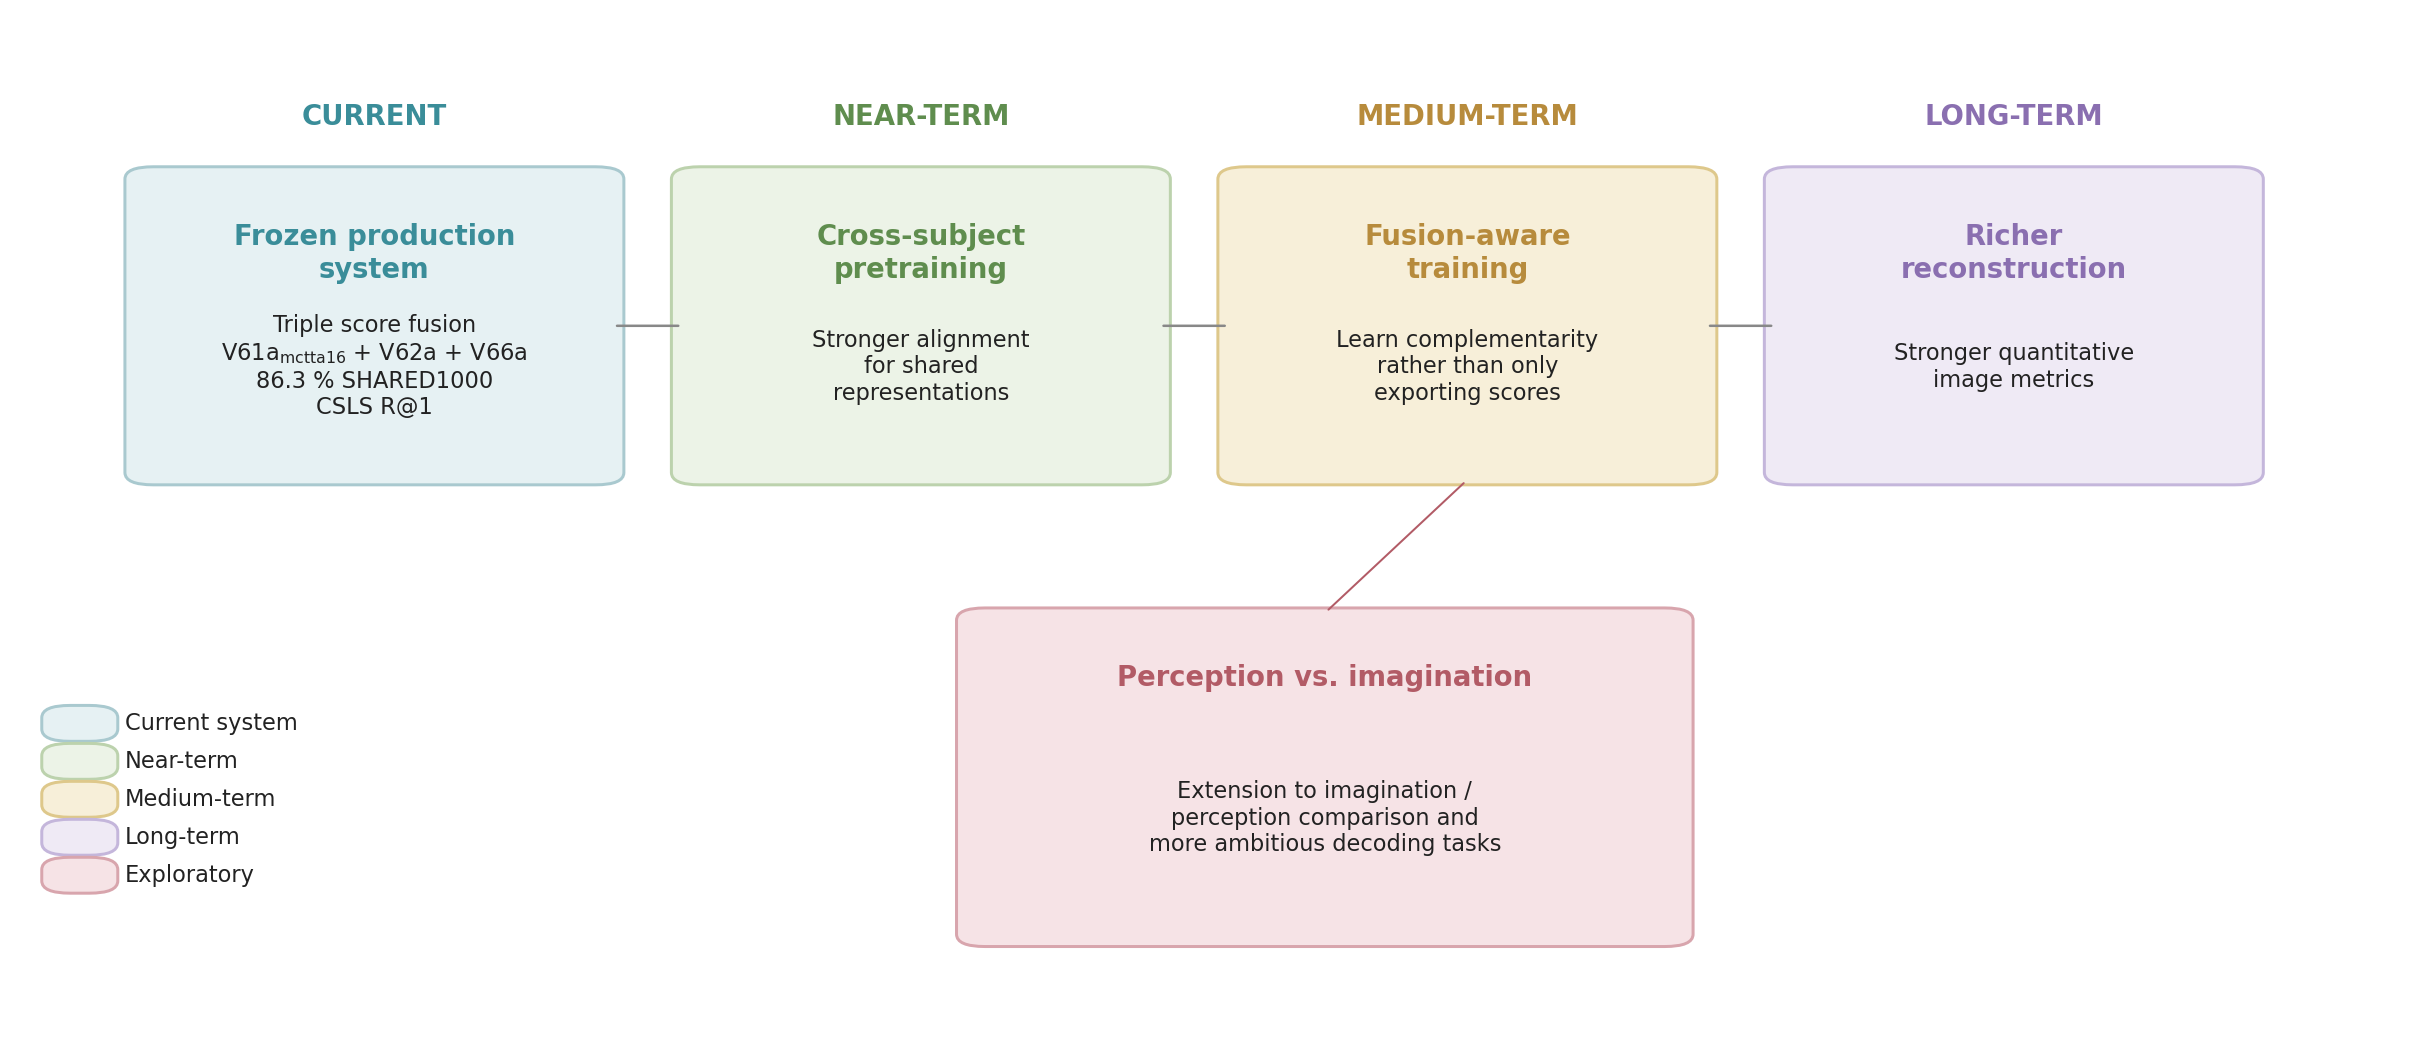
\includegraphics[width=\textwidth]{future_roadmap.png}
    \caption{Roadmap after the final triple-fusion retrieval system: stronger shared-subject alignment, fusion-aware training, more rigorous reconstruction evaluation, and broader perception-versus-imagery decoding.}
    \label{fig:future_roadmap}
\end{figure}
